 \documentclass[../Main.tex]{subfiles}
\begin{document}

Today we have a great variety of free open-source tools for NN purposes and its
number is increasing with the growth of AI and ML. Development of neural networks,
mobile application or server is full of nuances - an inexperienced programmer may 
encounter many troubles since not everything can be easily tracked. However, most
problems can be resolved by good Internet research. Therefore, it is highly significant
to choose the up-to-date tools with well-prepared documentation and active communities. 
Technologies we have chosen allowed us to focus on core concepts instead of 
struggling with implementation or configuration.

\subsection{Neural Network}

    \subsubsection{PyTorch}
        \textbf{PyTorch} is an open-source machine learning library created by Facebook and broadly used in the field of computer vision. Released in 2016 \cite{pytorch} rapidly gained popularity among researchers and developers. PyTorch is not another Python binding into a C++ framework. It uses core Python concepts like structures, classes or conditions, so integrates easily with the rest of Python ecosystem. Library provides all necessary tools for developing and training the neural networks based on deep learning models.
        
        Two main features of this package are:
        \begin{itemize}
            \item \textbf{Strong GPU acceleration} during computation of tensors
            \item Neural networks built on a tape-based \textbf{autograd system}
        \end{itemize}
        
        We decided to pick out PyTorch instead of TensorFlow (the main and actually the only alternative) due to several reasons. Firstly, TensorFlow was becoming more and more complex for machine learning beginners, where the PyTorch is based on basic and familiar programming paradigms. The new version of TF (2.0) solves this problem but was released  we had started working on the project. Moreover, the documentation is also pretty straightforward and helpful for newcomers. And finally, plenty of style transfer approaches are built on PyTorch. Including the network we adopt. 

    \subsubsection{CUDA}
    CUDA is parallel computing platform on GPUs and programming model created by NVIDIA \cite{cudatoolkit}. Using GPUs models can be train with shorter period of time and allow high floating-point computing performance.CUDA allows to use equivalent CPU functions for maximum use of GPUs and accelerate programms. Many frameworks like TensorFlow or PyTorch relay on CUDA for their GPU support. The NVIDIA company also created CUDA Toolkit, which includes libraries, debugging and optimization tool, which support all NVIDIA GPUs. There are three main libraries intended for deep learning CuDNN, which is the most popular for deep neutral network computations and mostly using in open source frameworks, TensorRT - the high-performance inference optimizer and runtime, and DeepStream, a library to video inference. You can use also use signal processing and math libraries. In case, when there are no needed library, you can write your low-level CUDA program in C or C++.  
%       \asia{add biblio:  --> dodane 
    
    \subsubsection{TensorRT} \label{trt_chapter}
    TensorRT is an SDK for deep learning interface \textbf{created by NVIDIA and designed for their GPUs}. It is built on CUDA and provides C++ and Python APIs, which allows loading pre-trained deep learning models, (trained with libraries like PyTorch) and run them on NVIDIA GPU. The main advantages of TensorRT are high-performance deep learning interface optimizer and light-weight runtime engine, that provide low latency and minimize streaming video delays \cite{tensorrtdocs}. The engine is generated only once for each GPU and serialized as a plan file for the next uses. It is also possible to run an application with lower precision (if hardware allows doing so) to reduce memory requirements and reduce inference time. 
    
    The workflow of the build phase network on TensorRT follows those steps:
    \begin{itemize}
        \item Eliminate layers with unused outputs
        \item Eliminate operation equivalent to no-operation
        \item Fusion of convolution
        \item Aggregation of operations with similar parameters on the same source tensor 
        \item Merge of concatenation layers
        \item Modifies the precisions of weights 
        \item Calibration and appropriate scaling factors
        \item Run layers on dummy data, to chose the fastest kernel catalog
    \end{itemize}
    
    TensorRT allows focusing on creating new applications with AI, autonomous machines
    and high-performance computing instead of calibration for inference development.
     optimization TensorRT chooses specific CUDA kernels for the platform to maximize
    performance on GPUs. It uses Docker for integration with DevOps architectures.\\
    TensorRT doesn't support direct building of engines from PyTorch models, so 
    we use ONNX format as intermediate step in build process. Specifically, after
    pruning we convert encoders, transformatiom module and decoder to ONNX. 
    ONNX tends to produce excessively complex computational graphs, which sometimes
    prevents from conversion to TensorRT, so next we use open-source ONNX simplifier 
    \cite{onnxsim} to make models more compact. Finally, using open-source
    onnx2trt parser \cite{onnx2trt} we build TensorRT engines based on simplified
    ONNX models.
    
%        \asia{add biblio: --> dodane

    \subsubsection{OpenCV}
    Open Source Computer Vision Library is an open-source library, originally developed by Intel, for computer vision and machine learning software \cite{opencvdocs}. It includes dozens of computer vision algorithms adjusted for easy use for detect and recognize faces, identify objects and many others designed for image processing. Although written in C++, OpenCV has Python bindings and provides support for Machine Learning libraries like PyTorch.  By using it, one can process images and videos to detect objects, apply filters, analyze structure or perform reconstruction. OpenCV is designed to handle real-time vision applications and is currently developing full-featured CUDA interfaces.

    \subsection{Distiller}
    Distiller\cite{distiller} is an open-source Python package for neural network compression.
    It provides a PyTorch environment for prototyping and analyzing compression algorithms,
    such as sparsity-inducing methods and low precision arithmetic. Distiller
    is still in experimental phase and is supposed to provide examples and tools
    to build your own pruning pipelines, rather than complex library of functions
    that would work of the box. As such it contains:
    \begin{itemize}
    \item A framework for integrating pruning, regularization and quantization algorithms
    \item A set of tools for analyzing and evaluating compression performance
    \item Example implementations of state-of-the-art compression algorithms
    \item Experimental implementations of knowledge distillation and conditional
          computation
    \item Convenient YAML format for describing compression schedule
    \end{itemize}
    We were particularly interested in available pruning algorithms.
    Out of many implemented methods only couple of them worked (that is threw easily
    fixable bugs). Considering results in \cite{li2016pruning} and comparisons
    in other papers we picked L1 structured pruning algorithm as a simple and reliable 
    method.

\subsection{Server}
    Client-server communication is divided into two parts: video streaming and transferring filter specification data. The first part is maintained by a server in WebRTC standard, whereas the second one is micro-server based on Flask. Both segments are written in Python and developed by open-source communities.

    \subsubsection{WebRTC}
    WebRTC is an open framework that enables \textbf{Real Time Communication (RTC)} in web browsers and mobile apps via simple API \cite{webrtc}. It provides tools to create peer-to-peer communication without any external plugins or programs. Standardized on API level by \href{https://www.w3.org}{W3C} and protocol level by \href{https://ietf.org}{IETF} is widely used and supported by Google, Apple, Microsoft, and main browser vendors. Given that our project and mobile application is cross-platfoom, we consider it as a key factor when choosing server technology.
    
    WebRTC architecture presented on  Figure \ref{fig:webrtc-public-diagram-for-website} contains two main layers: 
    \begin{itemize}
    \item C++ API - for browser makers implementing the Web API proposal
    \item Javascript Web API - for web developers building audio-video applications \\
    \end{itemize}
    
    \begin{figure}[h]
    \centering
    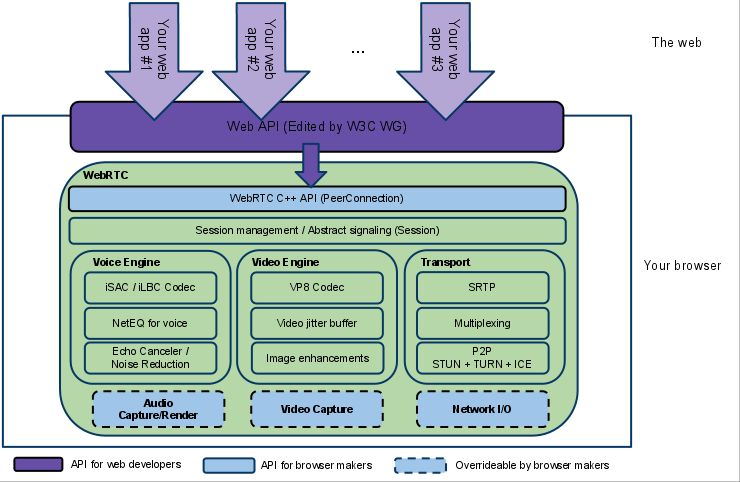
\includegraphics[width=0.7\textwidth]{webrtc-public-diagram-for-website}
    \caption{Overview of WebRTC architecture from official documentation \cite{webrtc}}
    \label{fig:webrtc-public-diagram-for-website}
    \end{figure}

    Comprehensive documentation and community creating many additional libraries make using this framework rather convenient. One of the most popular open-source libraries is \textbf{aiortc}.

    \subsubsection{Aiortc}
    \textbf{Aiortc} was developed as a 'WebRTC for Python' \cite{aiortcdocs}. Complexity (especially for beginners) and lack of Python bindings motivated authors of aiortc to design library and API which follow its Javascript counterpart. They pointed out that 
    'WebRTC (...) is tightly coupled to a media stack, making it hard to plug in audio or video processing algorithms' \cite{aiortcdocs}. 
    Our goal is to literally use the video processing algorithm, so we found this library and its examples extremely useful. We based our server on the aiortc example which performs video, audio and data channel establishing with a browser. It also allows pocessing streaming frames using OpenCV. 

    \subsubsection{Flask}
    Flask is a so-called \textbf{micro-framework} with little dependencies to external libraries, which provides tools and technologies useful with building a small web application \cite{flaskdocs}. It could be helpful for ones who want to create web pages, blogs or a simple REST server. 
    Technically, Flask is based on:
    \begin{itemize}
    \item Werkzeug WSGI (Web Server Gateway Interface is a popular specification for a universal interface between the  server and the web app) - toolkit which implements requests-response objects, and some service functions
    \item Jinja2 template engine - template system helpful with rendering dynamic web pages
    \end{itemize}
    Flask itself does not support database handling, validation or extensive visual templates. Being lightweight is the factor we found crucial, since our server does not perform any complicated tasks. Running constantly in the background, it only has to:
    \begin{itemize}
    \item Receive POST request from mobile application containing filter specification 
    \item Encode filter image and parameters
    \item Assign it to the IP of sender and store in particular folder
    \item Send confirmation response to the mobile app
    \end{itemize}
    We also decided to write simple Flask client in order to test connection to the server.

    \subsubsection{Server flow}
    The aforementioned servers work separately and do not directly interfere with each other and could perform tasks asynchronously. In that way, many clients can upload filter images and parameters as well as stream video without delays. Every client can change filter params and start a new stream in various order, but the usual client-server flow is depicted in Figure \ref{fig:server-flow} \\
    \begin{figure}[h]
    \centering
    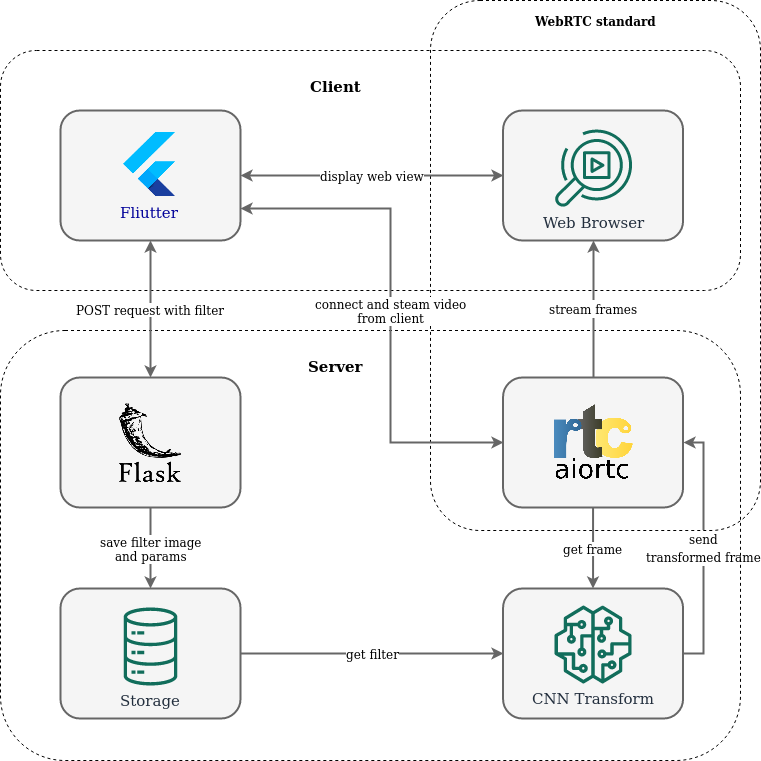
\includegraphics[width=0.7\textwidth]{server-flow}
    \caption{Client-server flow}
        \label{fig:server-flow}
    \end{figure}
    
    In a nutshell, when user selects filter style the following actions happen:
    \begin{enumerate}
    \item Mobile app send POST request to the Flask server running on port 5000 including JSON with three fields: filter image encoded in base64 format, filter benchmark value in float, boolean information about color preservation during process 
    \item Flask server performs tasks described in the section 5.2.3
    \item Mobile app ping server running on port 8080
    \item Server establishes RTC-peer connection with browser running inside app
    \item The stream is started - aiortc-based server catch frame and transform it using filter style image uploaded in advance from storage
    \item Transformed frame is added to RTC Media Stream Track and streamed back to the mobile browser
    \item Browser displays video using WebView component 
    \end{enumerate}
    
    When streaming finishes or breaks (due to network error, application shutdown or any other error), server close connection gracefully but still stores last filter style parameters. If they are not specified during the next stream or the POST request to the Flask server fails, the server uses saved ones. 
    
    \subsubsection{Alternative technologies}
    We had been trying several options before we chose to use aiortc. Our prime attempt was to adopt \href{https://github.com/cloudwebrtc/flutter-webrtc}{WebRTC Plugin for Flutter}. It is a small project developed by the Flutter community containing Javascript server and Flutter client. That seemed to be a perfect solution that could accelerate our work.
    However, we encounter some obstacles in this undertaking. First of all, the mentioned plugin is poorly documented and error-prone what is a rather annoying combination. Secondly, it works efficiently only over the LAN network when we wish to connect to the server from any place. And the third thing is the communication crashes if the video is not streaming to/from the Chrome browser. Nevertheless, the project is gathering greater community what makes it promising in the time of growing popularity of Flutter.

\subsection{Environment}
    Both model and server require multiple dependencies like:
    \begin{itemize}
        \item graphic card drivers
        \item python packages 
        \item Linux programs
        \item programs from Github
    \end{itemize}
    Even if we have all needed dependencies there still remains a problem with configuration which can take even hours. The target location of our program was one of the shared computers in Poznan University of Technology so we had to move the whole environment very quickly without making a mess. 
    Finally, we decided to put our application into Docker container to deal with all these problems.
    
    \subsubsection{Docker}
    Thanks to OS level virtualization Docker allows us to create containers where we can put our program and all its dependencies. We can have multiple containers and manage them easily using command line or one of the GUI clients, like \textit{Kitematic}. Docker containers are separated from each other so there is no risk to do harm to other containers or host. However, we can make our containers communicate by mapping some of container ports to host.
    
    Thanks to Docker containers we were able to pack everything up and deploy on university's computer.
    We put model, server, graphic card drivers, configuration files and all other dependencies into single container. Docker gives us the possibility to define whole building process in single file called \textit{Dockerfile}. During container building we can copy files from local drive, download programs from the Internet or even run bash scripts. 
    After having it built, we converted our container into image and uploaded it to \textit{Dockerhub} - a docker images library where everyone can upload their images. Last thing to do was just download image on computer and run graphic card configuration script which prepares software for used graphic card type.
    Project container is run with ports $8080$ and $5000$ mapped with same ports on host machine - on those ports both WebRTC and Flask servers are deployed. Client applications connecting to computer on these ports are in fact connecting with container.


\subsection{Mobile Application}
    This part describes the main technology used in clinet application which is Flutter. 
    We will also explain why we have chosen this specific technology.
    \subsubsection{Flutter}
        Today there are several frameworks which allows us to create mobile 
        applications for both Android and iOS simultaneously, 
        eg. React Native, Ionic, Xamarin.
        In 2015 Flutter joined this family and changed drastically situation
        on mobile application market. Nowadays, Flutter is the most popular multiplatform framework, which enables to 
        create not only mobile applications but also web from single codebase.
    
    
        Flutter is a framework created by Google but it's also an open source project 
        so everyone can propose new features and improvements. 
        When we write Flutter application we use Dart - language developed by 
        Google with C-style syntax.
        It runs on Dart VM included in the SDK. 
        A very interesting feature of Dart is that it optionally transcompiles to 
        JavaScript so you can also create web applications.
        
        
        Basic idea of Flutter sounds "Everything’s a widget" \cite{flutter-docs} and widgets are 
        quite similar to React "components". 
        They can be combined in order to create more complex ones. 
        The main purpose of widgets’ usage is to build a whole UI and some of them are:
        \begin{itemize}
            \item Layout widgets - e.g. rows, columns, lists, grids, tables
            \item Style widgets - e.g. colors, fonts
            \item Structure widgets - e.g. buttons, sliders, switches
            \item Animation widgets - e.g. transition, fade in
        \end{itemize}
        Flutter comes with loads of prebuilt Material Design and Cupertino(iOS style)
        widgets which makes easy and fast to create great looking applications. 
        There are Material Design icons, colors, typical UI interface 
        elements like top and bottom bars, buttons, list, animations and  many many more.
        
        
        Widgets are split into two main categories \cite{flutter-docs2}:
        \begin{itemize}
             \item Stateless - build only when the input data changes. 
             \item Stateful - build when input data or state property changes 
        \end{itemize}
        Difference between this two kinds of widgets is that the Stateless widgets
        never changes while Stateful ones can be modified during their lifetime.
        One of the examples of stateful widget is a simple checkbox. When we press checkbox
        it changes it's state to checked or unchecked and triggers rebuild on itself.
        When we want change to state of widget we must use special 
        \textit{setState} to made flutter re render this particular widget.
    
        
        Flutter architecture is composed of many layers \cite{flutter-docs} but we can divide it into 
        three main layers presented at Figure \ref{fig:flutter-layers}.
        \begin{figure}[h]
            \centering
            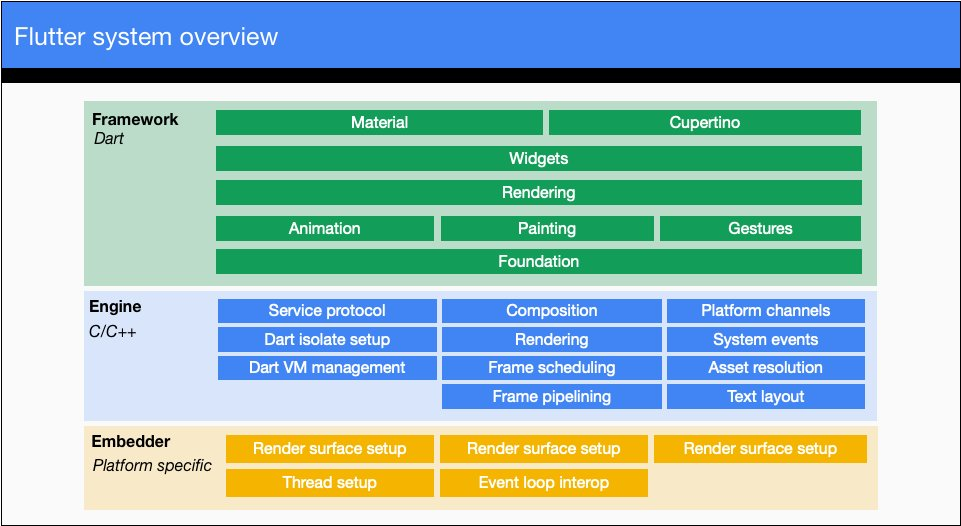
\includegraphics[width=0.80\textwidth]{flutter-system.jpeg}
            \caption{Flutter layers description \cite{flutter-docs}}
            \label{fig:flutter-layers}
        \end{figure}
        Programmers have more contact with top layers of framework - 
        these are Material and Cupertino widgets which are composed of basic widgets.
        Basic widgets use lower layers of framework. 
        The lowest one is foundation which contains core classes, functions and constants.
    
    
        From the beginning of our project we wanted to be able to develop new ideas
        very quickly.
        Python and PyTorch are technologies which definitely helped us keep high
        productivity during this time. First choose was Kotlin - a new modern programming 
        language for Android applications. Main advantages of Kotlin are:
            \begin{itemize}
                \item officially supported by Google
                \item high performance - native application
                \item some great language features like null safety, readability or async functions
                \item having an experience in this language
            \end{itemize}
            
        The main drawback of creating mobile applications with Kotlin is that creating
        some simple things can often take a lot of time as well as effort. 
        This was a main cause of rejecting this approach.
        We were looking for some other tools to create our client application and 
        eventually we found Flutter - relatively new tool framework from Google which 
        is still developing quite fast.
        The main advantage of Flutter is that we can develop your apps very 
        quickly as there are numerous efficient, ready-to-use and highly customizable 
        widgets. There is also a large community which creates new great widgets 
        add publishes them on official website so everyone can download them and use in project.
        You can also modify or build new widgets on the top of it and then publish.
        If some widget would become very popular and useful it will may be 
        include to official Flutter SDK. 
        Flutter also makes it easy to create apps in beautiful Material Design 
        style or its iOS equivalent - Cupertino. 
        The main feature of Flutter, which is always mentioned by Google is of course 
        creating applications for Android and iOS at the same time. 
        Our main goal was to create application for Android so we treated this feature like 
        an opened door. 
        Flutter is also declarative, react style framework which we prefer while
        creating user interfaces. We have had previous experience with React on web
        so Flutter seemed easy to learn. 
    

\biblio % Needed for referencing to working when compiling individual subfiles - Do not remove
\end{document}

